\chapter{You are one}
\addcontentsline{toc}{chapterdescription}{Who are you? Are you big enough? Understand why most self-help approaches don't work, or can even cause harm; and similarly for type indicators, declarations etc. Grow your subtlety in what you accept, what you rebel against, and how to be yourself with others. Expand your complexity of thought and meaning\hyp{}making stages, so that you are satisfied at the end when you measure your own life.}
\addcontentsline{toc}{chapterdescription}{\pagebreak}
\label{chapter:who-am-i-one}


\begin{chapterquotation}
People aren't just people, they are people surrounded by circumstances.\\
\raggedleft\textemdash Terry Pratchett\index{Pratchett, Terry} 
\end{chapterquotation}


\section{Who are you, are you big enough?}
\label{section:size-of-person}
You’ve maybe heard or read many times over that you cannot solve a problem with the same thinking that created it (Einstein).\index{Einstein, Albert}  In the language of this book, you cannot solve an adaptive challenge with the same Size of Person\index{Size of Person}  that created it.


In this book the phrase Size of Person (SoP) is your total three-dimensional capacity, as described in the previous three chapters: to fluidly use the 28 transformational thought forms; how far along the stages of meaning\hyp{}making you are; and your capacity to work subtly and wisely with your hardwired nature, including your capacity to manage your emotional state.


Figure~\ref{fig:ground-pattern} shows how the chapters of this part integrate. In it you can see how your behaviours are driven by your aspirational commitments (to achieve your goals) and your hidden commitments (to protect your vulnerabilities). Both of these are a consequence of who you are, including your nature and SoP. If your behaviours are blocking you from achieving your aspirational commitments, you have two options: either a Castle Move, an alternate behaviour that delivers simultaneously what your aspirational and hidden commitments need; or transformational experiments that chip away the invalid aspects of your meaning\hyp{}making stories.


\begin{figure}
\centering
    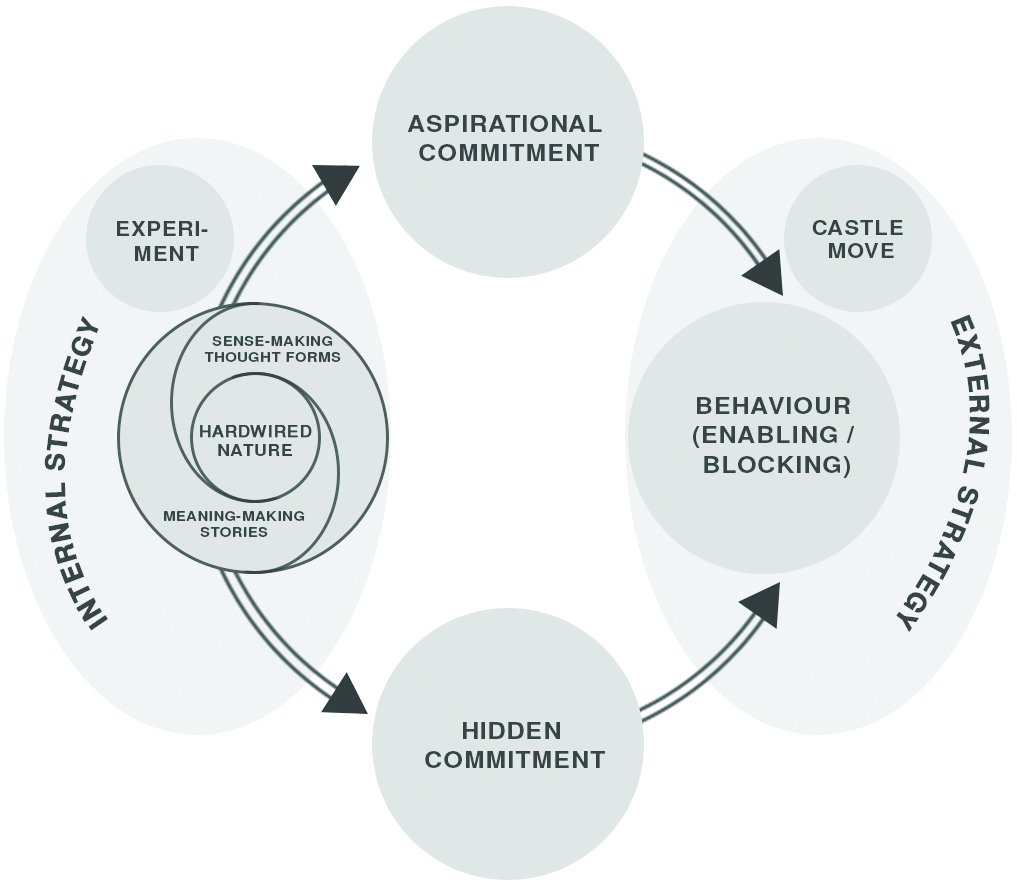
\includegraphics[width=0.95\textwidth]{./Images/Ground-pattern}
    \caption[How your sense-, meaning-making, and your nature drives your behaviours.]{How your inner SoP generates your experienced reality and drives your behaviour, as a competition between your commitments to achieve your aspirations and protect your vulnerabilities.}
    \label{fig:ground-pattern}
\end{figure}




I cannot emphasise enough that there is nothing inherently better or worse in having a bigger or smaller SoP. There is nothing inherently better, or to be proud of, in having your meaning\hyp{}making stories centred at a later stage in the sequence described in Section~\ref{section:dev-stages}. Just as an elephant is not inherently better than a virus.


The adaptive challenges we are facing are bigger than any challenge anyone has faced before. These challenges are as big as the planet, have time horizons of centuries, and are inherently nebulous, volatile, uncertain, complex, and ambiguous. Humanity needs enough people across all sizes of person to address them. 


Whoever you are and whatever your role, the bigger you are, the better you will rise to the challenge. Many are too small for these unprecedentedly large challenges, especially those experts who are at the expert intermediate stage of self-identity.\index{self-identity} 


The better you know the stories\index{stories}  that you use to shape your reality and give you your self-identity, and the better you are at then rewriting those stories, the more likely you are to shape a future reality that addresses the challenge.


The greater your fluidity in the 28 transformational thought forms,\index{thought forms (28)}  the more likely you are to be able to work with the irreducibly nebulous, complex, or even chaotic nature of the challenge without falling victim to harmful either / or logic. You will be able to apply the kind of thinking that transformed physics into quantum physics.\index{physics!quantum} 


The more subtlety you can use in rising above your own unique nature and biases, the more likely you are to address the challenge according to its actual nature, rather than according to your own.


In fact, I will go so far as to say that we would not have crossed the edge into our current climate emergency, nor any of the other existential crises humanity faces over the coming century, if the people who had shaped neoclassical economics\index{economics!neoclassical},  and applied it to our society, had been bigger. 


Today, none of us is big enough for the challenges we are facing. We need to grow.


\subsection{Sense-making}
\index{sense-making|(} 
In conversations that the two of us have had writing this book, about many economists and their research articles, we often come across evidence that they are not big enough for their work in the world. Especially they lack sufficient post-logical thinking capacity. 


If a thought form is not available to an economist, they won't see some aspect of the economy. All 28 thought forms of Chapter~\ref{chapter:who-am-i-sense} are \index{thought forms (28)} needed to really grasp the true significance of trends; what the signals visible ten years ago were telling us about today; and what the signals visible today are telling us about 50 years in the future.


Or consider a focus on data and formal manipulation of that data, rather than what lies behind the data. Your data is never neutral, your opinions on what matters, what data to gather, and how, shape the data before you even begin measuring. Your opinions come out of your meaning\hyp{}making stories\index{meaning-making stories}  and the thought forms you can use fluidly. And the better you get at recognising which stories and thought forms are shaping your opinions about which data you need, the more chance you have of recognising when you need completely different types of data. 


The essence of the scientific method is identifying opinions, and testing them, which makes clear how much in many of today's disciplines are more like the cargo cults described in Section~\ref{section:cargo-cults}.


If you are not fluid enough in the transformational thought forms, you may well be force-fitting your ungrounded opinion on the economy into logical right or wrong choices. It doesn't matter how precise your data is, if the thought forms you are using are insufficient to gather useful data and see clearly what you can and cannot use it for.


If you are highly fluid in these 28 thought forms, you'll be constantly aware that the economy is never absolute, it's always nebulous, because it is always under construction and, equally, your knowledge of it is always under construction and lagging behind the economy. \index{sense-making|)}


\subsection{Meaning-making and experts}
\index{meaning-making|(} 
Too many experts, economists\index{economists}  included, use just one lens\index{lens} in making meaning and only one frame of reference\index{frames of reference} in evaluating. In Chapter~\ref{chapter:who-am-i-meaning} you read about the different stages of meaning making that human beings can go through in sequence. Later stages allow you to grasp different types of stories,\index{stories} and to create your own stories with less and less dependency on the stories of others.


One stage that may well partly cause the distrust that many have for experts is the expert stage halfway between S3 and S4, Chapter~\ref{chapter:who-am-i-meaning}. Recall, if you are at this stage, you make meaning and shape your reality based on others recognising you as an expert. So any challenge to your discipline means an identity crisis.


In physics,  it took a couple of decades for quantum physics\index{physics!quantum}  to establish itself as a new domain of expertise, and so a group for socialised mind and expert stage folk to derive their identity from. The people who were able to move first were those who had progressed beyond the expert stage. Over time, they formed a new group that others could join as expert members, while those who could not eventually retired and left active work in physics.


A big driver of your meaning making, in addition to the stage that your meaning\hyp{}making stories are at, are the different cognitive biases described in Section~\ref{section:biases}. 
The Dunning-Kruger effect (imposter syndrome), \index{Dunning-Kruger effect} or inferiority-superiority bias, \index{biases} authority bias, consistency bias, and uncertainty avoidance bias all have a significant effect on anyone who is sought out as an expert, and wearing a label of authority like professor or consultant or executive.


The book \emph{The Econocracy: The Perils of Leaving the Economy to the Experts}\cite{earl-econocracy} points\index{The Econocracy}  very clearly at the impact of too small SoP\index{Size of Person}  individuals in positions of power over others and the discipline. 


The authors refer to the economics profession as an elite, disconnected from the rest of us and our day-to-day use of our economy as a tool to do the job of provisioning\footnote{The Econocracy is one of many tangible and transformational outcomes that emerged from the global dissatisfaction, beginning around 2001, of economic students with the validity of what they were being taught.}. The emergence of such an elite is often a consequence of a large enough community of people whose sense of self-esteem and identity comes from shared stories of being experts recognised and validated by the other experts in the field. 


Very much as in Ubuntu (section~\ref{section:ubuntu}), \index{Ubuntu} this becomes a self-reinforcing closed community. Any challenge to the expertise is identical to a challenge to the identity of the community as a whole, and specifically any individual that is challenged.


This is a stage that every professional discipline goes through as it evolves and that a number of human beings go through. Applying thought forms T1, 2, 3, and 4, this is \index{thought forms (28)} nothing other than the necessary conflict and loss of stability necessary to transform the economics discipline to the next stage with the adaptive capacity capable of rising to our crises. Embrace the tension and conflict, it's your friend!\index{conflict} 


You can do this, if you remind yourself every time you feel triggered at a challenge to your expertise, that this challenge has got nothing to do with you, or your legitimacy to have expertise. The strength of your trigger is most of the time simply valuable data telling you about deeply hidden meaning\hyp{}making stories that you are using to construct your self-identity.


So economics\index{economics}  is today at the same exciting time that physics\index{physics} was a century ago; on the edge of an equivalent great shift to the shift from classical to quantum. To leap across the chasm between economics as it has been, and economics as it will be, economics needs big economists, just as physics needed big physicists. 


If your work includes balancing and coordinating across multiple systems, for example multiple institutions across the economy, politics, and society, you need to be big. Else the Dunning-Kruger effect \index{Dunning-Kruger effect} may well bite you!


\begin{longstoryblock}
I (Jack) would not be here writing this book with Graham without the following response to a paper that I submitted to a peer-reviewed journal early in my career. Even though the reviewer’s response was clearly painful for me, with hindsight I can see how the meaning\hyp{}making story shaped the reality of my life.


I had discovered an error in the deductive logic of a fundamental model in neoclassical economics. Not knowing anything about the expert stage of identity, I naïvely assumed that my discovery would be welcomed by the economics discipline, so we could correct an error and move forward. My worst ‘fear’ was that somebody would point out the logical error that I had made, which I would’ve welcomed, since it would have made me a better economist.


Instead, I received a terse, three-word letter of  rejection: 


\begin{quote}
How dare you! 
\end{quote} 


I asked myself what is wrong with the economics discipline if a very simple question on the internal logical consistency of a small building block of economic theory generates a thermonuclear emotional response.  


(I wish I had then known how my meaning\hyp{}making stories and the referee's meaning\hyp{}making stories created the reality that each of us experienced.)


I was buoyed by the always-helpful advice of my football (American) coach, Frank deFelice:


\begin{quote}
Success is defeat turned inside out.
\end{quote}


Indeed, I turned this defeat into success by sketching on the back of the rejection letter, a new story that would (hopefully) transform the economics profession and how we educate our economists. This new story created, three years later, the first edition of \emph{The International Journal of Pluralism and Economics Education}.


In 2015 I was invited to speak at the Rethinking Economics Conference in London, because of my research work and as the journal’s founding editor; I met Graham, and this book is the consequence.


This book that you are now reading never would have happened without that rejection letter, and so if you derive any benefit from reading this book, then that rejection letter may well have been the best thing that ever happened to me.


Take hope that your journey and the difference you can make in the world will be bigger and quicker than the journeys Graham and I have had to get to this point. You're building on everything in this book, and in the books listed in our bibliography, and much more. You're bringing your own genius to play, surfing on a rising tide of many more. Ubuntu\index{Ubuntu} at work again. 
\end{longstoryblock}




Every successive improvement and expansion in quantum physics \index{physics!quantum} has described even better what we see happening in nature. Regardless of which philosophical interpretation a physicist finds most plausible, all physicists\index{physicists} use the same equations and make the same predictions of what will happen. Predictions that have consistently proven extraordinarily accurate.


It's high time that we develop the same rigour in our studies and paradigms of business and economics. We may never be able to pin down which is the right interpretation of what an organisation is or is for, but if we manage to get the same experimental rigour into business and economics, we will at least know what works. 


The way forward is to repeat what physicists did a century ago. Recognise that the different philosophies of quantum physics primarily exist so that we can feel secure in our meaning making. As soon as physicists only focused on using quantum physics to make smartphones, GPS devices, and many other products that we depend on today, all physicists agreed.


We need to get to that point in business and economics.\index{economics} Way too much still depends on opinions that have as much anchoring in what actually works in organisations and businesses as the air anchoring the clouds I'm currently looking at above the mountain across the valley.
\section{Who you are now vs. who you are}
\label{sec:who-am-i}
Recall, from Section~\ref{section:ergodicity}, that most of our economy is non-ergodic, even though most of economics assumes ergodicity. As we introduced there, this has huge implications for who you are, and what it means to “find oneself”.


Who you are is the integration of every influencing event in your experienced reality along your life path; which may well go back a number of generations. It's not for nothing that many ancient customs take into account seven generations. Think: \emph{I am my life path and the meaning-making stories that I have internalised because of that life path.} 


Who you are not a static thing. So you never can “find yourself” and then stay true to that self forever, unchanging. Nor ought you put your life on hold until you have found yourself. Because who any of us is is a process across time, not a static thing in the here and now. Who you are is continuously being changed through your relationships with others and your environment. You are an open dynamic system in constant transformation. (This applies all the thought forms of Chapter~\ref{chapter:who-am-i-sense} to see your self across, rather than in, time.)


Who you are now is the integration of your entire life path within your experienced reality up to now: every influence, every experience you have made meaning of; and, to make matters even more challenging, also the integration of your expectations about your life path into the future.


You truly are unique.


No-one else has had your life path ever before, nor will any one else ever have your life path again. 


And since that is common for everyone, around 8 billion people, it also means you are also not unique! You being unique and not unique is yet another complementary pair.


So often we all limit ourselves by looking at ourselves in the moment through a narrow lens that excludes almost all of who we are across all time, saying something like \emph{I am a \ldots}; and then identifying who we are with those words\textemdash across all time, all people, and all situations.


Equally we often delude ourselves that we are far more than we are in exactly the same way!


Any self-declaration in time beginning with \emph{I am \ldots}, and any declaration another makes about you beginning with \emph{You are \ldots} cannot precisely describe all that you are across time.


This life path perspective is missing in most approaches to identity and belonging. Identity groupings (e.g., gender, culture, nationality, etc.) of people around some common ground at a point in time (the present, or some past milestone) have validity; and yet miss the uniqueness integrating each individual’s entire life path across time.


Some of you may identify with some past milestone, e.g. where you’ve come from (\emph{I was born a \ldots and so I am a \ldots, but you were not, and so you are not part of my identity group}); or maybe with where you are now (\emph{I say I am a \ldots; you also say the same; so we’re the same, and are members of my identity group}). Both of these lenses on self-identity have full validity within one frame of reference, and neither is complete in all frames. Each emphasises one aspect of common ground by hiding complementary aspects of uniqueness, and common ground with others. 


And so arguments between people and members of an identity grouping about someone \emph{being a \ldots or not} usually produce only emotions, seldom understanding, let alone resolution, because they fail to see how those differences and similarities are created by the lenses used and the narrow focus on one characteristic, at one time, rather than each person’s full being across time. 


You are a unique integration of your life path to now and into the future. 


And you have multiple types of common ground with many other people. Choose for yourself the groups you identify with.


And you have some common ground with everyone alive today, with everyone who has ever lived, and with everyone who ever will live.


Coming back to the crises of today then. Whoever you are now, however you evaluate yourself, and however daunting your journey may seem, I see two reasons to stay hopeful.


\begin{itemize}
\item Whoever you think you are after reflecting on those questions and reading this book, you're already far more than that. None of us ever can be fully aware of everything that we are. We are always more aware of part of who we are, and unaware of some other part. You are a lot like a Picasso painting, there's always far more to you than whatever you are currently seeing.
\item Also, like quantum physics\index{physics!quantum}, as soon as you focus your awareness on yourself, you immediately change yourself. Who you are, as you become aware of yourself, has already changed. So who you think you are is always one step behind who you are. I find that a very powerful reason to hope that I am already someone even more able to rise to the adaptive challenges I am choosing to face, and already even more someone that I will enjoy spending the rest of my life with.
\end{itemize}


Remember, you are unique. 


No-one else experiences the same reality you experience, and so no-one else can be who you can be. 


And who you are being can continue to change, as it has changed so far, so that you can be who your world needs you to be.


\section{Why most self-help approaches aren’t helpful}
\label{section:empiricism}


To change your being, you may turn to one of the many self-help approaches. Some work, some do not, and some cause harm. 


For example, the Losada ratio of flourishing people having three to six times more positive emotions than negative, often cited in positive psychology, is wrong\cite{sokal-losada-wrong}. Mindfulness, which does good for many, can also cause harm\cite{farias-buddha}. People have ended up needing to be hospitalised because of mindfulness training. Many self-help approaches are like the cargo cults of Section~\ref{section:cargo-cults}\textemdash they have similar visible rituals to ones that work, but lack the hidden engines.


All approaches to development and growth need to be treated with a high level of self-aware caution. Including everything in this book. 


\subsection{Declarations don't work}
One recurring theme in self-help\index{self-help} is pumping yourself up. Self-help is full of admonishments to look yourself in the mirror each morning and say something like \begin{quote}Every day, in every way, I'm getting better and better.\end{quote} 


Look at some well-known, popular programmes built around a charismatic individual exhorting you to tell yourself you can do it, and making good money for their founders and key staff members; even though their foundation is luck, not a method that works\cite{wilson-redirect} to drive change. And even worse, some are so flawed they are actively harmful. 


A very effective route to going under in the turbulent stresses of modern life is simplistically declaring that you are awesome, instead of the hard but effective work of dismantling the scripts that tell you otherwise, then using experiences in the areas you do well in, and those you do not, so the scripts rewrite themselves. 


If most self-help actually worked, there would be few people trying out a new technique every year. The self-help industry protects itself, because the implicit mantra is, \emph{if you failed to help yourself, it is your fault, because you didn’t do it right}. 


The whole industry of self-help,\index{self-help} weight-loss, motivation etc. is filled with approaches that, in themselves, are inherently incapable of delivering reliable, long-lasting benefit. Only a few lucky people experience long-lasting benefits. Lucky, because the benefits come from some other cause than the self-help approach. 


But because the industry has become so good at persuading you that failure is your fault, not theirs, the response of most people is to blame themselves, and then buy another book or course. 


You can read a lot more about why most approaches at best do no good, and often do harm, apart from those that involve you recognising and changing your stories in \emph{Redirect} by Timothy Wilson\cite{wilson-redirect} \index{Wilson, Timothy} and \emph{SHAM: How the Self-Help Movement Made America Helpless} by Steve Salerno\cite{salerno-sham}.\index{Salerno, Steve}


The empirical evidence for what really works, without risk of harm, and that leads to sustainable growth and transformation, shows that it is all in the meaning\hyp{}making stories that shape our thoughts, our feelings, and trigger our actions; and our fluidity in transformational thought forms.


To change or improve yourself, it's no good to just counter-declare yourself to be different to who your stories\index{stories} declare you to be. Counter-declaring like this can cause harm. 
\subsection{Typologies need a pinch of salt}
\label{section:against-typologies}


Type indicators have become popular over the past couple of decades. I recommend that you avoid all type indicators with fixed categories, such as the MBTI and Enneagram. Many are a modern equivalent to the cargo cultists: they look evidence-based, they give you an illusion of understanding, a feel-good factor, but that's all. 


There is growing evidence that these type indicators are too generic to be really useful\cite{vermeren-undesired-popularity-of-typologies}, let alone help you grow into who you can become. Rather, you shape yourself to fit into whichever box a test has put you into. If you end up believing, and adopting as your own, the meaning\hyp{}making stories of a specific MBTI or Enneagram category, you may well narrow and slow down your development towards \emph{your} next meaning\hyp{}making stage.


More recent approaches do not allocate you to a box with a label, but rather tell you how high or low you score on a few dimensions. One example of this is the OCEAN (Openness, Conscientious, Extroversion, Agreeableness, Neuroticism) set of traits. 


These have a usefulness as a language to communicate clearly within your inner dialogue and with others. OCEAN is now well-validated, but, no matter how validated, they (including everything in this book) are limited, because no model can never capture the full nebulous, unknowable being that you are. 


So reject all type indicators and profiles that claim to tell you who you are\textemdash yet have all 7.9 billion unique human beings in just a few boxes. Take all with a pinch of salt, some with a couple of tonnes. Each of us is unique. There is no one else just like you. 




\subsection{Why coaching can stunt your development}
Much coaching\index{coaching} is surface-level behavioural: it is there to change your behaviours so that you can achieve your aspirational commitments. Or, far worse, so that you can achieve someone else's goals, often your boss’s. 


Behavioural coaching based, not on castle moves, but only on simplistic attempts to change your blocking behaviours without understanding the vital role they are playing in protecting vulnerabilities in your big assumptions, and without understanding the developmental process that you go through as you progress from one meaning\hyp{}making stage to the next.


So whilst you may temporarily succeed in delivering your immediate goal, your vulnerability is likely to feel more threatened, and come back with an even stronger way of protecting itself. That will simply hold you back even more from your next goal, and from developing yourself into who you are intended to become. It will hold you back from becoming authentic.


You are also likely to end up feeling even more stressed, and in even greater need of coaching. A wonderfully self-perpetuating business model, if ever I saw one. 


Too few coaches out there are sufficiently fluid in all 28 thought forms, especially the specific transformational thought forms T1 to T7. A coach must have sufficient fluidity and stage of development in their own open meaning\hyp{}making system to effectively and safely engage with your open, transforming meaning\hyp{}making system.


Just as you saw that S4 is the earliest category of meaning making sufficiently independent of the need to belong to a group and follow its norms to be able to manage others, so too is S4 is the earliest category able to coach another as a different but equal being.


If you are being coached by someone with less fluidity than you have, or at a less complex stage of meaning\hyp{}making, your coach's smaller capacity is more likely to just pull you back to their SoP. Only a coach with a bigger SoP\index{Size of Person} than you can support you to grow your SoP.


So choose your coach with a high degree of caution. If your gut instinct suggests that they don't get you, or they are misinterpreting as resistance your attempts to pin down and clarify a nebulous sense that something is wrong in their understanding of you, it may be time for a new coach. 


Of course, sometimes you will be wrong. Sometimes Dunning-Kruger \index{Dunning-Kruger effect} is at work, and you are simply not yet big enough to grasp what the coach is doing. Sometimes your own psychological idiosyncrasies are creating an inner reality that is so distorted from actuality that you cannot see clearly.


This is why I believe that the best approach to development is through your work, in a structured peer-to-peer dialogue, using a common language and patterns, with your colleagues or peers, e.g. the Adaptive Way\index{Adaptive Way} (strictly applying the three rules of safety: care for yourself; care for each other; care for the whole). This is also the only approach that can scale to reach enough people in the decade we have left to build the regenerative businesses and the regenerative economy needed to address our global crises.


As the old maps\index{maps} used to say, proceed with caution, for there be dragons ahead. But only by proceeding can you tell whether these are the beneficial dragons of some Asian cultures, or the threatening dragons of European cultures.


\section{Self-protection}
Never forget that you have every right to protect yourself. You will live with the consequences of your choices of who to follow; which practice to incorporate into your life; who to allow into your life as mentor, coach, or guru.


Keep in mind, about 1\% of the population has narcissistic personality disorder, another 1\% has strong psychopathic tendencies. What better job for them to find prey than providing professional help? Keep your eyes open.


Apply the PT Barnum test\cite{wiseman-paranormality} to anything or anyone that in any way is attempting to tell you who you are. Much in the typologies, the self-help industry, spiritual development, astrology etc. fails the PT Barnum test.\index{PT Barnum test} 


The Barnum test captures how easy it is to write a description that appears to be specific about a few people, and yet that most people believe accurately describes them. This has been demonstrated time and again in research. In the first study, a paragraph (like those you find in type indicators) was given to a full cross-spectrum of university students of all types and natures. They were asked to rate this for how accurately it described them, on a scale from 1 (not at all) to 5 (this is absolutely and uniquely me). The average was 4.3. 


This shows how easy it is to write or say something that looks specific, but is in fact so general that it fits many extremely well. These are the kinds of things used by people who want you to feel special, or to manipulate you; and that are behind some type indicators, and more.


We are all very easy to fool, especially those of us trained in the sciences. We learn to think that everything is rational and, whilst nebulous, is never malicious. Stage magicians are often a far more reliable judge than scientists of whether something is a con, playing on our human capacity for deception, or for real. Listen to them too! 


Deeply mistrust any mystical explanation of some phenomenon, if the same phenomenon can be reproduced by a magician using sleight of hand and misdirection.


Protect yourself by keeping in mind that you are the only person who can ever have the depth and breadth of understanding to define who you are, let alone who you ought to become. 


\emph{Certainly no colleague or manager has the capacity, let alone the right, to play God: to attempt to define who you are or should be.} 


Anyone who says to you anything beginning with \begin{quote} you are \ldots (annoying, lazy, clever, kind, successful) \end{quote} may well be playing God over you. Even if they are just saying that as a colloquial form of expressing their personal admiration, rephrase it. What they are actually saying is that their meaning\hyp{}making stories attribute this quality to what they are seeing of you. Whilst they are saying it’s about you, it's actually more about them.


I recommend that you read \emph{Experiencing the Impossible: The Science of Magic} by Gustav Kuhn\cite{kuhn-magic}, \emph{Paranormality} by Richard Wiseman\cite{wiseman-paranormality}\index{Wiseman, Richard} and \emph{The Buddha Pill} by Miguel Farias\index{Farias, Miguel} and Catherine Wikholm\cite{farias-buddha} to get an even better idea of the different ways you can be fooled, and what you can do to protect yourself.\index{Kuhn, Gustav}\index{Wikholm, Catherine}


For me, the bottom line is that it is \emph{my} life, \emph{my} experienced reality generated through \emph{my} meaning\hyp{}making stories\index{meaning-making stories} that I have to live with. I choose.








\section{Accepting or rebelling against who you are}
Your very first job in life, from the moment you were born, was to grow up into the biggest, shiniest self that you could become. This job stays with you throughout your life. Your primary job is to be yourself, and continue to grow into who you can become, in this nebulous, VUCA world.\index{VUCA} 


\emph{Accept} and work subtly with everything that seems to be part of your unchangeable core essence. It is as futile for you to try to change that, as it was when King Canute deliberately demonstrated the futility of even a King trying to hold back the tide. Part of your unchangeable core essence includes, for example, sounds you can distinguish easily but others cannot (e.g. \emph{l} vs. \emph{r}), and even emotions you can experience, but others cannot, because the environment, including beliefs and culture, you grew up in, as well as your early childhood experiences, gave you a different neural connectivity to another. 


\emph{Rebel} against any part of you that is not part of your core essence and is creating a distorted experienced reality contrary to your core essence, or that is taking you down a path towards long-term harm.


Your real challenge, as you undoubtedly know, is how on earth are you going to tell the difference? Unfortunately, there is no easy way. This has always  been a challenge for each of us and will remain a challenge for the rest of our lives. I have found it useful to combine constant experimentation, using improv\index{improv} to try out different possible steps for me to take in my development, moving forwards with whatever seems to work, and never taking anything as right.


Picasso's art, as on the cover, is relevant to this.\index{Picasso, Pablo} There is no right perspective to take in deciding who you ought to become, and there is no single you that you ought to become. You are a flowing river, not a static thing. Like his art, there are infinitely many possibilities ahead for you to become. Of course, there are limitations and boundaries.\index{boundaries} You cannot become someone that is contrary to your core, unchangeable essence. But within that space, you have infinite possibility.


This story of my journey may help you by illustrating what I'm talking about.
\begin{longstoryblock}
I (Graham) have tried to gain weight, and especially to put on more muscle. From around 10 years old until around 40 I tried everything I could. Multiple different eating regimes, different exercise routines, heavy weights with few repetitions, light weights with lots of repetitions, rowing, cycling, rock climbing, the works. 


None of them led to sustained weight gain. I have always been a tall skinny guy. 


The driver behind all this effort was a deep assumption that I was not OK as I was. Recall, I grew up in South Africa\index{South Africa}, where sport and physical prowess is the most highly prized quality at school. Even more so, I went to a boys-only school, where sporting achievement was the route to respect and acceptance from my peers. So from a very young age I learnt that until I had muscles and excelled at sport, I was nothing. 


Now I've given up trying to gain weight. I've ceased blaming myself for not trying hard enough, because I now know two things. First, the stories I believed are not true everywhere, always, with everyone. I have respect because of who I am in total, regardless of how much muscle that total includes. Secondly, there are unchangeable limits to how much muscle I can gain. My body is what it is. 


Believing that I could have the body I wanted if I tried hard enough, and therefore, it was my fault for not trying hard enough, was just setting myself up for failure. Now my attention is focused on right health, which means eating and exercising well. I have accepted that that means staying at a lightweight 67~kg at 6~ft~2" height. 


Even more, I have transformed myself by re-writing my stories. Now I am proud that, at 55, I am as slender and healthy as I was at 20. The only physical issues I now have are back and knee injuries\textemdash ironically caused by training beyond my nature’s limits, with weights that were simply too heavy for me.
\end{longstoryblock}


Treat yourself with at least as much compassion and kindness as you would anyone that you cared deeply for. Most of us, though, find it extraordinarily difficult to see ourselves through such a lens\index{lens} of compassion and kindness, and refuse to allow ourselves to simply be what is deeply embedded in our nature, and unchangeable.


The better you get at applying the quote from Reinholdt Niebuhr on page~\pageref{quote:niebuhr}, the better you will be able to harness the unique strength that your nature gives you, and the less you will waste those strengths in futile rebellion against the weaknesses that they bring with them.


All the patterns in this book, and in all the forthcoming books, are useful in enabling you to do that. Stop bullying yourself, and instead accept with kindness and compassion your nature. Stop bullying yourself, and instead explore your meaning\hyp{}making stories, and then create experiential experiments so that they rewrite themselves.
\section{Being yourself with others}
\label{section:dressed}


I find the quote by Terry Pratchett at the start of this chapter a very neat way of describing the philosophy of Ubuntu (Section~\ref{section:biases}), and what we discovered in Section~\ref{section:dressed-you}, that you always show up as your dressed self.


You cannot switch your self-awareness on or off consciously. (I use awareness and consciousness\footnote{In my opinion, consciousness is simply the emergent property of a fantastically complex system, our huge brain of neurons, neurotransmitters, etc. I find myself in awe of just how much more must be possible in this universe, if a sufficiently complex constellation of protons, neutrons and electrons is able to be aware of itself and understand protons, neutrons and electrons.} as nearly synonymous.) Once you have become aware of something, you cannot actively become unaware. Equally, if you have no awareness, you lack even the awareness to begin the journey to becoming aware.


What is currently in your self-awareness changes slightly your self-identity, because it changes which of your stories is in the driving seat. Since you cannot decide now to shut down your awareness of yourself. It’s a bit like telling someone 
\emph{now whatever you do, do not, under pain of death, think of a pink elephant}. The very attempt to not to think of the pink elephant is itself a thought of a pink elephant, and so they think of and see a pink elephant. (Every time I edited this I ended up seeing a pink elephant too.)


Because you are self-aware, your self-identity\index{self-identity} in any instant is “fully dressed”. It's the self you get after all the different elements of your self-awareness have acted on each other. 


In that sense, you are actually never your “naked” self. You are always the you after all the bias and distortions coming from your self-awareness have done their work. It means that who you are is always under construction, never ever fixed. 


You can take huge hope from this because it means that you can make some very easy changes. Just changing what in yourself you are aware of already begins to change your self-identity. 


If you are in the grip of anger with a colleague and become aware of this, you change, and anger loses some of its grip on you. Then becoming aware that you are much more than your anger; that you have anger now in this moment, which is quite different to seeing your being as angry, loosens the grip even more. Step even deeper into awareness that your colleague is also far more than just a target for anger, they are everything a colleague can be, including at this moment one who has done something that triggers anger in you.


Then suddenly you’ve regained your self-identity as a fully conscious human being, and are aware of your colleague as another different but equally fully conscious human being. You’ve stepped from a smaller self-identity into a bigger one. 


Notice how this is exactly what I recommend you use to prevent being manipulated through your biases\index{biases} in Section~\ref{section:biases}


This also means that Ubuntu~\ref{section:ubuntu} acts on an individual level, as well as at a societal level.\index{Ubuntu} 


\begin{longstoryblock}
I (Graham) show up quite differently with two different work associates. With one, I'll call him Mike, I usually feel calm, energised and optimistic. With the other, I'll call her Sarah, for a long time I felt energised as well, but also frustrated and irritable. With Sarah, at first I tried working on my stories. What was it in my stories that was reacting to what she was doing? I tried various experiments, I tried various improv approaches, I tried everything described in Part~\ref{part:you} and more. Nothing worked, nothing changed, increasing my frustration and irritation every time we worked together.


Through a process of elimination, it became clear to me that what was happening lay neither just in me, nor just in her. Most of what was happening lay in the archetypal relationship between someone with my essence and category of stories, and someone with her essence and category of stories. 


The relationship exists independently of us, shaping each of us; who I am and who she is in that relationship is shaped by this third, independent entity, the relationship. By recognising that the dressed me is created by the relationship, and the dressed Sarah is also created by the relationship, it made it very clear that, for me to change how I was showing up, and the reality that I was experiencing, it was essential for her to change herself, so that both of our dressed selves became different. Then a different type of relationship could emerge, reinforcing our changed selves.


I realised just how much of who I was, was there because of who she was, and that neither of us were to blame. This enabled me to look at Sarah and myself with a high level of acceptance and compassion. With the balance and peace that that gave me, I took the steps to change the kind of work we were doing together to one that would enable us both to be effective, given the reality that each of us shapes for ourselves in response to the other person.
\end{longstoryblock}


Keep this firmly in mind when you are working with your colleagues. If there is someone who frustrates or angers you, maybe it's neither them, nor you. Maybe they are only this way with you, and you are only this way with them. So don't blame yourself, and don't try to fix yourself, in isolation. In the same way, don’t blame the other person, and don’t try to fix them, in isolation. Each of you is shaping each of you through the kind of relationship that has you in its grip. You will learn a pattern called deconstructive conflict in Section~\ref{section:deconstructive-criticism}, \index{conflict!deconstructive} which is the most powerful pattern I have ever found to enable you to transform who you are, and your relationships at work.


Recall what I wrote in Section~\ref{section:optimised-self}. The meaning\hyp{}making stories that shape who you are your superpower versus all other life forms on the planet. Even more powerfully, the stories of a tribe, a sports club, or the community of people that constitute a business, are their collective superpower.


Human beings could never collaborate the way we do, to overcome challenges that are bigger than any single human being, without the collective stories that unite us. These collective stories enable us to see the common oneness that unites us. 


Just as in quantum physics, where no particle is an independent isolated entity, but rather where the properties of every single particle are shaped by every other particle around it and shape every particle around it, your personal stories create the collective stories of the groups of people you are part of and are in turn shaped by the collective stories.


There is no way of teasing apart your story from the collective story.


Nor should you ever try to. This is a core message behind applying the lessons of quantum physics\index{physics!quantum} and Picasso's \index{Picasso, Pablo} art to ourselves. If you try to separate yourself from everyone and everything around you, if you try to separate your story from our stories, you will lose the very superpower that you need to overcome the challenges that you, and we, will face in the next ten years.


When we are with others, we tend to put ourselves into boxes, we put other people into boxes, and none of those boxes are ever all you are. The better you understand your stories, the better you get at guessing the stories that are running somebody else, the better you'll get at recognising when your way of being and meaning\hyp{}making have put somebody into a box. \emph{Leadership and Self-Deception}, an excellent book\cite{arbinger-leadership} by the Arbinger Institute\index{Arbinger Institute} expands fully on this. 


If you read it after reading this book, you may suspect what I suspect: that their “in-the-box” is what I would call S3 meaning\hyp{}making, and their “out-of-the-box” is what I would call stepping into the bigger box of S4. Since S4 is just a bigger box, you may need to step out again into the next bigger box of S5, and then into the even bigger box of S6. So you are always in a box\textemdash the question is, is it big enough for the task at hand?
\section{Bigger than one: from you and me to us}
Each of us is part of a much bigger whole than any of us can easily imagine. We are one life out of countless many living organisms on one bluish planet revolving at 19 miles per second around a sun that provides us with all the energy that almost all life on the planet uses.


For most of human history, life demanded far less from the planet and it’s limits. We have now grown so big that we have hit the limits to growth\cite{rome-limits}. We've hollowed out Kate Raworth's\index{Raworth, Kate} doughnut\cite{raworth-doughnut} until no dough is left, only us nuts.


A thread throughout life, that I hope is clearly visible throughout this book, is that what we all have in common with all other human beings, and all life on the planet, is far bigger than the dominant logic of today sees. This common oneness is far more important in each of us being able to survive and thrive than the uniqueness of any of us.


To move forward, we now need an Ubuntu philosophy to take centre stage, rather than an individualistic philosophy.


Once we do this, we will start multisolving\cite{sawin-multisolving}\index{multisolving}, as Elizabeth Sawin\index{Sawin, Elizabeth} of Climate Interactive has named those single actions that simultaneously solve multiple problems. For example, replacing a coal-fired power station with a combination of photovoltaic panels on everyone's roofs, wind turbines nearby, and local storage of electricity in the form of hydrogen, compressed air, or any other form, is multisolving.


It contributes towards solving our climate emergency\index{climate!emergency}, and it solves health issues, reducing the burden on health insurance and medical practitioners of the many problems caused by pollution. It increases the lifespan of our buildings by reducing the impact of pollution, including acid rain. It reduces local unemployment and poverty by providing work that is best done by large numbers of small businesses rather than one big power plant, and so on.


The better we are at using all 28 thought forms, \index{thought forms (28)} at recognising that the common ground that unites us is far more important than the uniqueness that divides us and that all our problems are interrelated, the easier it gets for us to find one quick and affordable action that is a multisolution.


We cannot see everything that a multisolution will solve until after the fact, but just knowing that they exist and that we can find them is part of what gives me hope.


One organisation that Evolutesix\index{Evolutesix} has supported, including incorporating it as a FairShares Commons,\index{FairShares Commons} is UniOne. UniOne\index{UniOne} is a business and a movement that provides safe spaces where wide ranges of differently unique people can come together and stand safely in their common oneness and, at the same time, without any loss of self, in their diverse individual uniqueness.


This is at its most powerful when highly diverse unique organisations and cultures find a way to come together and collaborate on the common oneness because they retain the full power of their individual uniqueness. Until nations and their politicians can do this sufficiently well, we are unlikely to move forward on the political contributors to our global crises.


Until different businesses can do this, we are unlikely to move forwards on the business contributors. But at least we have now ways of incorporating that make this natural, like the FairShares Commons.


\section{How will you measure your life?}
Take a moment to imagine that you are now at the end of your life. Maybe only the end of your working life, or the end of whatever phase of your life you are in now. 


Sitting there at your life’s end, looking back, how will you measure your life?


This is the topic of the excellent book\cite{christensen-measure} by Clayton Christensen,\index{Christensen, Clayton} aptly entitled \emph{How will you measure your life?}, which strongly influenced me (Graham) in 2009 when I first read it, and the  Adaptive Way. The book is based on the lecture he gives to his business school class at the end of every year, where he shows how to apply everything that he has taught about business strategy and disruptive innovation\cite{christensen-dna} to oneself.


I recommend that you sit down, perhaps at the end of every year, and imagine that you are sitting at life’s end. You are now looking back over your life and measuring it. How will you measure it? Which measures, or frames of reference, will you use? What evaluation will you give to your life? What were the major choices you made, the important actions you took, that created this life?


You will likely be tempted to do this in the present, writing about what you will do. Avoid that. Seat yourself firmly in the future, at the end of your life, and write as if you had already done it. (See \emph{giving an A} in \emph{The art of possibility}\cite{zander-art}.)


Think about which measures, or frames of reference, are really important to you now. Think about how they may change from now until the end. And then take that as the best set of measures you can use now as you imagine yourself measuring your life.